\documentclass[tikz, border=3.14mm]{standalone}
\usepackage{pgfplots}
\pgfplotsset{compat=1.18}

\begin{document}
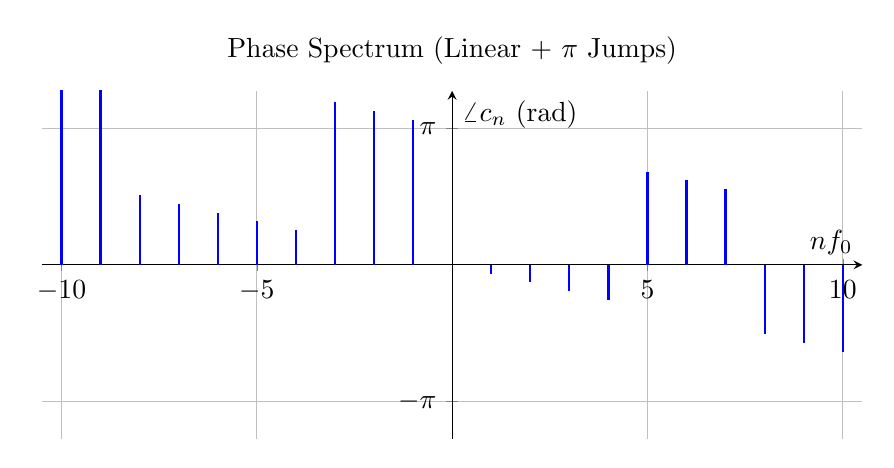
\begin{tikzpicture}
    \begin{axis}[
        axis lines = middle,
        xlabel = {$n f_0$},
        ylabel = {$\angle c_n$ (rad)},
        xmin = -10.5, xmax = 10.5,
        ymin = -4, ymax = 4,
        xtick = {-10, -5, 0, 5, 10},
        ytick = {-3.1415, 0, 3.1415},
        yticklabels = {$-\pi$, 0, $\pi$},
        grid = major,
        width = 12cm,
        height = 6cm,
        title = {Phase Spectrum (Linear + $\pi$ Jumps)}
    ]
        % Linear phase part: -n*w0*(t0 + tau/2)
        % Plus pi jumps when Sa(x) < 0
        % Let's assume t0 + tau/2 results in a slope of -0.2
        % Sa(x) crosses zero at n = 4, 8, ...
        
        \addplot[blue, thick, ycomb, samples at={-10,-9,...,10}] {
            (-0.2*x) + ( (sin(3.1415*x*0.25*180/3.1415) < 0) ? 3.1415 : 0 )
        };
        
        % Wrap it to [-pi, pi] if needed, but linear shows the drift better
        
    \end{axis}
\end{tikzpicture}
\end{document}
